% This is auto-generated file: do not edit!
% Exported from microMathematics Plus, version 2.17.1


Esse exemplo demonstra como calcular
séries e integrais.

\subsection{Taylor series}

Na matemática, séries de Taylor são uma
representação de uma função como uma
soma infinita de termos que são
calculados a partir da derivada dos
valores da função num único ponto.

Por exemplo, Ts(x,N) é a expansão de
Taylor de uma função com argumento x e
N número de termos:
\begin{center}\begin{tabular}{c}
  $Ts(x,N) := \displaystyle\sum_{n=0}^{N} \frac{{ \left( -1\right) }^{n}}{\left( 2 \cdot n \right)! } \cdot {x}^{2 \cdot n}$
\end{tabular}\end{center}

Esta expansão se aproxima da função
cosseno:
\begin{center}\begin{tabular}{c}
  $s(x) := cos \left( x\right) $
\end{tabular}\end{center}

Se desenharmos as duas funções juntas
para o mesmo intervalo, elas parecem
iguais:
\begin{center}\begin{tabular}{c}
  $x := \left[ 0,\, 0.1 \,..\, 2 \cdot {\pi} \right]$
\end{tabular}\end{center}
\begin{center}\begin{tabular}{c} 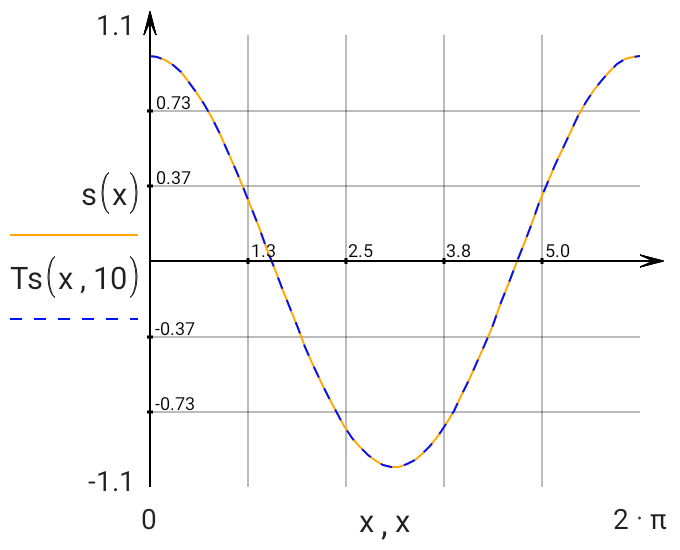
\includegraphics[resolution=320]{graphics/series_and_integrals_fig1.png} \end{tabular}\end{center}

Entretando, há um erro numérico devido
ao número limitado de termos de
aproximação N. A função a seguir
$\Delta$(x,N) descreve este erro:
\begin{center}\begin{tabular}{c}
  ${\Delta}(x,N) :=  \left| s \left( x\right)  - Ts \left( x,\, N\right)  \right| $
\end{tabular}\end{center}

Podemos desenhar esta função em
coordenadas logarítmicas e ver que o
erro numérico diminuirá se tivermos
mais termos na soma de Taylor:
\begin{center}\begin{tabular}{c}
  $E(N) := log10 \left( {\Delta} \left( {\pi},\, N\right) \right) $
\end{tabular}\end{center}
\begin{center}\begin{tabular}{c}
  $N := \left[ 3,\, 4 \,..\, 13 \right]$
\end{tabular}\end{center}
\begin{center}\begin{tabular}{c} 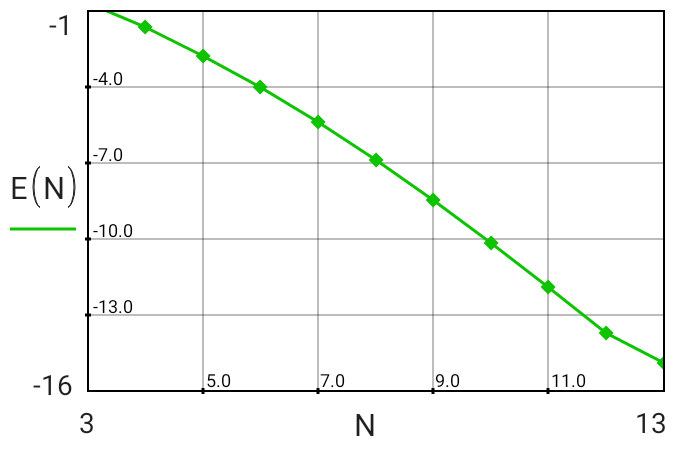
\includegraphics[resolution=320]{graphics/series_and_integrals_fig2.png} \end{tabular}\end{center}

\subsection{Série Binomial}

Consideremos esta função potência:
\begin{center}\begin{tabular}{c}
  $f(x,{\alpha}) := {\left( 1 + x \right)}^{{\alpha}}$
\end{tabular}\end{center}

Esta função pode ser aproximada usando
Série Binomial:
\begin{center}\begin{tabular}{c}
  $Tf(x,{\alpha},N) := \displaystyle\sum_{n=0}^{N}  \left( \displaystyle\prod_{k=1}^{n} \frac{{\alpha} - k + 1}{k}\right)  \cdot {x}^{n}$
\end{tabular}\end{center}

Podemos também desenhar as duas funções
(a função de potência dada e sua
aproximação) juntas no mesmo gráfico:
\begin{center}\begin{tabular}{c} 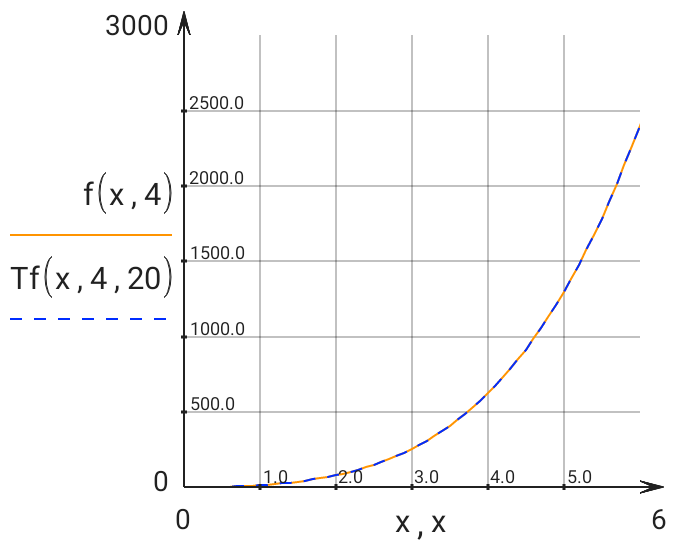
\includegraphics[resolution=320]{graphics/series_and_integrals_fig3.png} \end{tabular}\end{center}

\subsection{Integrais}

Também é possível calcular uma integral
definida numericamente usando o método
de Simpson. Por exemplo, podemos
calcular a integral usando o elemento
''Visualização de resultado'':
\begin{center}\begin{tabular}{c}
  $\displaystyle\int_{0}^{3 \cdot pi / 2}{cos \left( \frac{2 \cdot x}{9}\right) }^{-2}\, dx = 7.79423$
\end{tabular}\end{center}

A solução analítica é
\begin{center}\begin{tabular}{ccc}
  $I := \frac{9 \cdot \sqrt{3} }{2}$ &
  ,    &
  $I = 7.79423$ \cr
\end{tabular}\end{center}

O erro numérico pode ser calculado
como:
\begin{center}\begin{tabular}{c}
  $\displaystyle\int_{0}^{3 \cdot pi / 2}{cos \left( \frac{2 \cdot x}{9}\right) }^{-2}\, dx - I = 4.26681E-9$
\end{tabular}\end{center}

Este erro depende do valor de ''Número
de dígitos significativos no
resultado'' que pode ser alterado na
janela ''Configurações do Documento''
disponível a partir da barra de ações:
\begin{center}\begin{tabular}{c} 
\includegraphics[resolution=320]{graphics/series_and_integrals_fig4.png} \end{tabular}\end{center}

Se este valor aumentou, o limiar que
controla a precisão do método de
Simpson também aumentará.